\documentclass[twoside]{book}

% Packages required by doxygen
\usepackage{fixltx2e}
\usepackage{calc}
\usepackage{doxygen}
\usepackage[export]{adjustbox} % also loads graphicx
\usepackage{graphicx}
\usepackage[utf8]{inputenc}
\usepackage{makeidx}
\usepackage{multicol}
\usepackage{multirow}
\PassOptionsToPackage{warn}{textcomp}
\usepackage{textcomp}
\usepackage[nointegrals]{wasysym}
\usepackage[table]{xcolor}

% Font selection
\usepackage[T1]{fontenc}
\usepackage[scaled=.90]{helvet}
\usepackage{courier}
\usepackage{amssymb}
\usepackage{sectsty}
\renewcommand{\familydefault}{\sfdefault}
\allsectionsfont{%
  \fontseries{bc}\selectfont%
  \color{darkgray}%
}
\renewcommand{\DoxyLabelFont}{%
  \fontseries{bc}\selectfont%
  \color{darkgray}%
}
\newcommand{\+}{\discretionary{\mbox{\scriptsize$\hookleftarrow$}}{}{}}

% Page & text layout
\usepackage{geometry}
\geometry{%
  a4paper,%
  top=2.5cm,%
  bottom=2.5cm,%
  left=2.5cm,%
  right=2.5cm%
}
\tolerance=750
\hfuzz=15pt
\hbadness=750
\setlength{\emergencystretch}{15pt}
\setlength{\parindent}{0cm}
\setlength{\parskip}{3ex plus 2ex minus 2ex}
\makeatletter
\renewcommand{\paragraph}{%
  \@startsection{paragraph}{4}{0ex}{-1.0ex}{1.0ex}{%
    \normalfont\normalsize\bfseries\SS@parafont%
  }%
}
\renewcommand{\subparagraph}{%
  \@startsection{subparagraph}{5}{0ex}{-1.0ex}{1.0ex}{%
    \normalfont\normalsize\bfseries\SS@subparafont%
  }%
}
\makeatother

% Headers & footers
\usepackage{fancyhdr}
\pagestyle{fancyplain}
\fancyhead[LE]{\fancyplain{}{\bfseries\thepage}}
\fancyhead[CE]{\fancyplain{}{}}
\fancyhead[RE]{\fancyplain{}{\bfseries\leftmark}}
\fancyhead[LO]{\fancyplain{}{\bfseries\rightmark}}
\fancyhead[CO]{\fancyplain{}{}}
\fancyhead[RO]{\fancyplain{}{\bfseries\thepage}}
\fancyfoot[LE]{\fancyplain{}{}}
\fancyfoot[CE]{\fancyplain{}{}}
\fancyfoot[RE]{\fancyplain{}{\bfseries\scriptsize Generated by Doxygen }}
\fancyfoot[LO]{\fancyplain{}{\bfseries\scriptsize Generated by Doxygen }}
\fancyfoot[CO]{\fancyplain{}{}}
\fancyfoot[RO]{\fancyplain{}{}}
\renewcommand{\footrulewidth}{0.4pt}
\renewcommand{\chaptermark}[1]{%
  \markboth{#1}{}%
}
\renewcommand{\sectionmark}[1]{%
  \markright{\thesection\ #1}%
}

% Indices & bibliography
\usepackage{natbib}
\usepackage[titles]{tocloft}
\setcounter{tocdepth}{3}
\setcounter{secnumdepth}{5}
\makeindex

% Hyperlinks (required, but should be loaded last)
\usepackage{ifpdf}
\ifpdf
  \usepackage[pdftex,pagebackref=true]{hyperref}
\else
  \usepackage[ps2pdf,pagebackref=true]{hyperref}
\fi
\hypersetup{%
  colorlinks=true,%
  linkcolor=blue,%
  citecolor=blue,%
  unicode%
}

% Custom commands
\newcommand{\clearemptydoublepage}{%
  \newpage{\pagestyle{empty}\cleardoublepage}%
}

\usepackage{caption}
\captionsetup{labelsep=space,justification=centering,font={bf},singlelinecheck=off,skip=4pt,position=top}

%===== C O N T E N T S =====

\begin{document}

% Titlepage & ToC
\hypersetup{pageanchor=false,
             bookmarksnumbered=true,
             pdfencoding=unicode
            }
\pagenumbering{alph}
\begin{titlepage}
\vspace*{7cm}
\begin{center}%
{\Large Solve\+Square }\\
\vspace*{1cm}
{\large Generated by Doxygen 1.8.13}\\
\end{center}
\end{titlepage}
\clearemptydoublepage
\pagenumbering{roman}
\tableofcontents
\clearemptydoublepage
\pagenumbering{arabic}
\hypersetup{pageanchor=true}

%--- Begin generated contents ---
\chapter{File Index}
\section{File List}
Here is a list of all files with brief descriptions\+:\begin{DoxyCompactList}
\item\contentsline{section}{\hyperlink{_solve_square_8cpp}{Solve\+Square.\+cpp} }{\pageref{_solve_square_8cpp}}{}
\end{DoxyCompactList}

\chapter{File Documentation}
\hypertarget{_solve_square_8cpp}{}\section{Solve\+Square.\+cpp File Reference}
\label{_solve_square_8cpp}\index{Solve\+Square.\+cpp@{Solve\+Square.\+cpp}}
{\ttfamily \#include $<$stdio.\+h$>$}\newline
{\ttfamily \#include $<$math.\+h$>$}\newline
Include dependency graph for Solve\+Square.\+cpp\+:\nopagebreak
\begin{figure}[H]
\begin{center}
\leavevmode
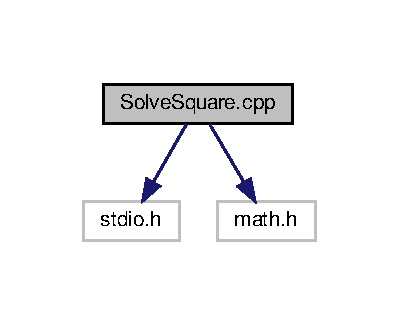
\includegraphics[width=192pt]{_solve_square_8cpp__incl}
\end{center}
\end{figure}
\subsection*{Solve\+Square}
\label{_amgrp1b1d7a37e4dd10b388093083b79136ec}%
\begin{DoxyVersion}{Version}
1 
\end{DoxyVersion}
\begin{DoxyAuthor}{Author}
Ivan Shargin, phystech 
\end{DoxyAuthor}
\begin{DoxyDate}{Date}
11.\+10.\+18 
\end{DoxyDate}
\begin{DoxyCompactItemize}
\item 
const int \hyperlink{_solve_square_8cpp_ae831e56053b8abc343b931bc11a63be4}{I\+N\+F\+I\+N\+I\+TE} = -\/1
\begin{DoxyCompactList}\small\item\em Substitute of infinity. \end{DoxyCompactList}\item 
const int \hyperlink{_solve_square_8cpp_a776a0d25487aee09ec4693cb6c6c6e3d}{S\+T\+R\+A\+N\+G\+En\+Roots} = -\/2
\begin{DoxyCompactList}\small\item\em Error code associated with invalid number of roots. \end{DoxyCompactList}\item 
int \hyperlink{_solve_square_8cpp_a89de4c22b83bf0121b8b28dacb08278a}{Get\+Coefficients} (double $\ast$a, double $\ast$b, double $\ast$c)
\item 
int \hyperlink{_solve_square_8cpp_ab2dd9b24e0e487efdd1cd1f40dd3a023}{Solve\+Square} (double a, double b, double c, double $\ast$x1, double $\ast$x2)
\item 
int \hyperlink{_solve_square_8cpp_afbeb15c6aba7bd93cfefddb22ffb7ff3}{Solve\+Linear} (double b, double c, double $\ast$x)
\item 
int \hyperlink{_solve_square_8cpp_ae66f6b31b5ad750f1fe042a706a4e3d4}{main} ()
\end{DoxyCompactItemize}


\subsection{Function Documentation}
\mbox{\Hypertarget{_solve_square_8cpp_a89de4c22b83bf0121b8b28dacb08278a}\label{_solve_square_8cpp_a89de4c22b83bf0121b8b28dacb08278a}} 
\index{Solve\+Square.\+cpp@{Solve\+Square.\+cpp}!Get\+Coefficients@{Get\+Coefficients}}
\index{Get\+Coefficients@{Get\+Coefficients}!Solve\+Square.\+cpp@{Solve\+Square.\+cpp}}
\subsubsection{\texorpdfstring{Get\+Coefficients()}{GetCoefficients()}}
{\footnotesize\ttfamily int Get\+Coefficients (\begin{DoxyParamCaption}\item[{double $\ast$}]{a,  }\item[{double $\ast$}]{b,  }\item[{double $\ast$}]{c }\end{DoxyParamCaption})}

Gets coefficients of quadratic equation from console. If it\textquotesingle{}s format is invalid, give new chance to enter coefficients. 
\begin{DoxyParams}[1]{Parameters}
\mbox{\tt out}  & {\em a,b,c} & coefficients of quadratic equation a$\ast$\+X$^\wedge$2 + b$\ast$X + c = 0 \\
\hline
\end{DoxyParams}
\mbox{\Hypertarget{_solve_square_8cpp_ae66f6b31b5ad750f1fe042a706a4e3d4}\label{_solve_square_8cpp_ae66f6b31b5ad750f1fe042a706a4e3d4}} 
\index{Solve\+Square.\+cpp@{Solve\+Square.\+cpp}!main@{main}}
\index{main@{main}!Solve\+Square.\+cpp@{Solve\+Square.\+cpp}}
\subsubsection{\texorpdfstring{main()}{main()}}
{\footnotesize\ttfamily int main (\begin{DoxyParamCaption}{ }\end{DoxyParamCaption})}


\begin{DoxyParams}[1]{Parameters}
\mbox{\tt in}  & {\em a,b,c} & Coefficients of quadratic equation a$\ast$x$^\wedge$2+b$\ast$x+c=0. \\
\hline
\mbox{\tt out}  & {\em x1,x2} & First root, second root of equation. If there is only one root, program uses x1. \\
\hline
\mbox{\tt in}  & {\em n\+Roots} & Number of roots. \\
\hline
\end{DoxyParams}
\mbox{\Hypertarget{_solve_square_8cpp_afbeb15c6aba7bd93cfefddb22ffb7ff3}\label{_solve_square_8cpp_afbeb15c6aba7bd93cfefddb22ffb7ff3}} 
\index{Solve\+Square.\+cpp@{Solve\+Square.\+cpp}!Solve\+Linear@{Solve\+Linear}}
\index{Solve\+Linear@{Solve\+Linear}!Solve\+Square.\+cpp@{Solve\+Square.\+cpp}}
\subsubsection{\texorpdfstring{Solve\+Linear()}{SolveLinear()}}
{\footnotesize\ttfamily int Solve\+Linear (\begin{DoxyParamCaption}\item[{double}]{b,  }\item[{double}]{c,  }\item[{double $\ast$}]{x }\end{DoxyParamCaption})}

Solve linear equation. 
\begin{DoxyParams}[1]{Parameters}
\mbox{\tt in}  & {\em b,c} & Coefficients of linear equation b$\ast$X + c = 0 \\
\hline
\mbox{\tt out}  & {\em x} & Root of equation \\
\hline
\end{DoxyParams}
\begin{DoxyReturn}{Returns}
Number of roots 
\end{DoxyReturn}
\mbox{\Hypertarget{_solve_square_8cpp_ab2dd9b24e0e487efdd1cd1f40dd3a023}\label{_solve_square_8cpp_ab2dd9b24e0e487efdd1cd1f40dd3a023}} 
\index{Solve\+Square.\+cpp@{Solve\+Square.\+cpp}!Solve\+Square@{Solve\+Square}}
\index{Solve\+Square@{Solve\+Square}!Solve\+Square.\+cpp@{Solve\+Square.\+cpp}}
\subsubsection{\texorpdfstring{Solve\+Square()}{SolveSquare()}}
{\footnotesize\ttfamily int Solve\+Square (\begin{DoxyParamCaption}\item[{double}]{a,  }\item[{double}]{b,  }\item[{double}]{c,  }\item[{double $\ast$}]{x1,  }\item[{double $\ast$}]{x2 }\end{DoxyParamCaption})}

Solve quadratic equation (a$\ast$\+X$^\wedge$2 + b$\ast$X + c = 0) if a!==0 or calls function Solve\+Linear if a==0. 
\begin{DoxyParams}[1]{Parameters}
\mbox{\tt in}  & {\em a,b,c} & Coefficients of equation a$\ast$\+X$^\wedge$2 + b$\ast$X + c = 0 \\
\hline
\mbox{\tt out}  & {\em x1,x2} & Roots of equation \\
\hline
\end{DoxyParams}
\begin{DoxyReturn}{Returns}
Number of roots 
\end{DoxyReturn}


\subsection{Variable Documentation}
\mbox{\Hypertarget{_solve_square_8cpp_ae831e56053b8abc343b931bc11a63be4}\label{_solve_square_8cpp_ae831e56053b8abc343b931bc11a63be4}} 
\index{Solve\+Square.\+cpp@{Solve\+Square.\+cpp}!I\+N\+F\+I\+N\+I\+TE@{I\+N\+F\+I\+N\+I\+TE}}
\index{I\+N\+F\+I\+N\+I\+TE@{I\+N\+F\+I\+N\+I\+TE}!Solve\+Square.\+cpp@{Solve\+Square.\+cpp}}
\subsubsection{\texorpdfstring{I\+N\+F\+I\+N\+I\+TE}{INFINITE}}
{\footnotesize\ttfamily const int I\+N\+F\+I\+N\+I\+TE = -\/1}



Substitute of infinity. 

\mbox{\Hypertarget{_solve_square_8cpp_a776a0d25487aee09ec4693cb6c6c6e3d}\label{_solve_square_8cpp_a776a0d25487aee09ec4693cb6c6c6e3d}} 
\index{Solve\+Square.\+cpp@{Solve\+Square.\+cpp}!S\+T\+R\+A\+N\+G\+En\+Roots@{S\+T\+R\+A\+N\+G\+En\+Roots}}
\index{S\+T\+R\+A\+N\+G\+En\+Roots@{S\+T\+R\+A\+N\+G\+En\+Roots}!Solve\+Square.\+cpp@{Solve\+Square.\+cpp}}
\subsubsection{\texorpdfstring{S\+T\+R\+A\+N\+G\+En\+Roots}{STRANGEnRoots}}
{\footnotesize\ttfamily const int S\+T\+R\+A\+N\+G\+En\+Roots = -\/2}



Error code associated with invalid number of roots. 


%--- End generated contents ---

% Index
\backmatter
\newpage
\phantomsection
\clearemptydoublepage
\addcontentsline{toc}{chapter}{Index}
\printindex

\end{document}
